\chapter{Vlastní implementace vybraných kompresních algoritmů}

\section{Technická specifikace}
\subsection{Vývojové prostředí a programovací jazyk}
Na základě osobních preferencí jsem zvolil programovací jazyk C\# verze 5.0, který poskytuje sofistikované a otestované nástroje pro práci s XML i JSON, a vývojové prostředí Microsoft Visual Studio Ultimate 2013, které poskytuje plnou podporu pro práci se zvoleným jazykem.

Dalšími použitými nástroji jsou framework NUnit verze 2.6 pro účely testování, ReSharper 8.0.1 pro správu testů a refaktorování\footnote{Refaktorování je proces úprav kódu vedoucí ke zlepšení jeho struktury, ale nemající vliv na funkčnost.} a verzovací systém Git, jehož podpora je ve Visual Studiu přímo implementována.

\subsection{Implementace a testování}
Při implementaci jednotlivých algoritmů jsem postupoval metodou vývoje řízeného testy (aglicky Test Driven Development). Při té programátor nejprve napíše neprocházející test, který definuje výchozí a požadovaný stav, a až poté implementuje logiku tak, aby test prošel. Díky vhodně napsané sadě testů je možné velice rychle a snadno odhalit chybu při další implementaci nebo refaktorování.

\subsection{Projekt}
Výstupem mé práce je knihovna tří vybraných kompresních algoritmů. Její struktura je zobrazena na obrázku \ref{strukturaKnihovny}. Každému algoritmu odpovídá jedna příznačně pojmenovaná třída, jejíž veřejné rozhraní poskytuje metody \texttt{Compress} a \texttt{Decompress}. Tyto metody na vstupu očekávají cestu k souboru, který má být zpracován, a po úspěšném zpracování všech dat na stejném umístění vytvoří soubor s komprimovanými/dekomprimovanými daty.

\begin{figure}[!h]
\centering
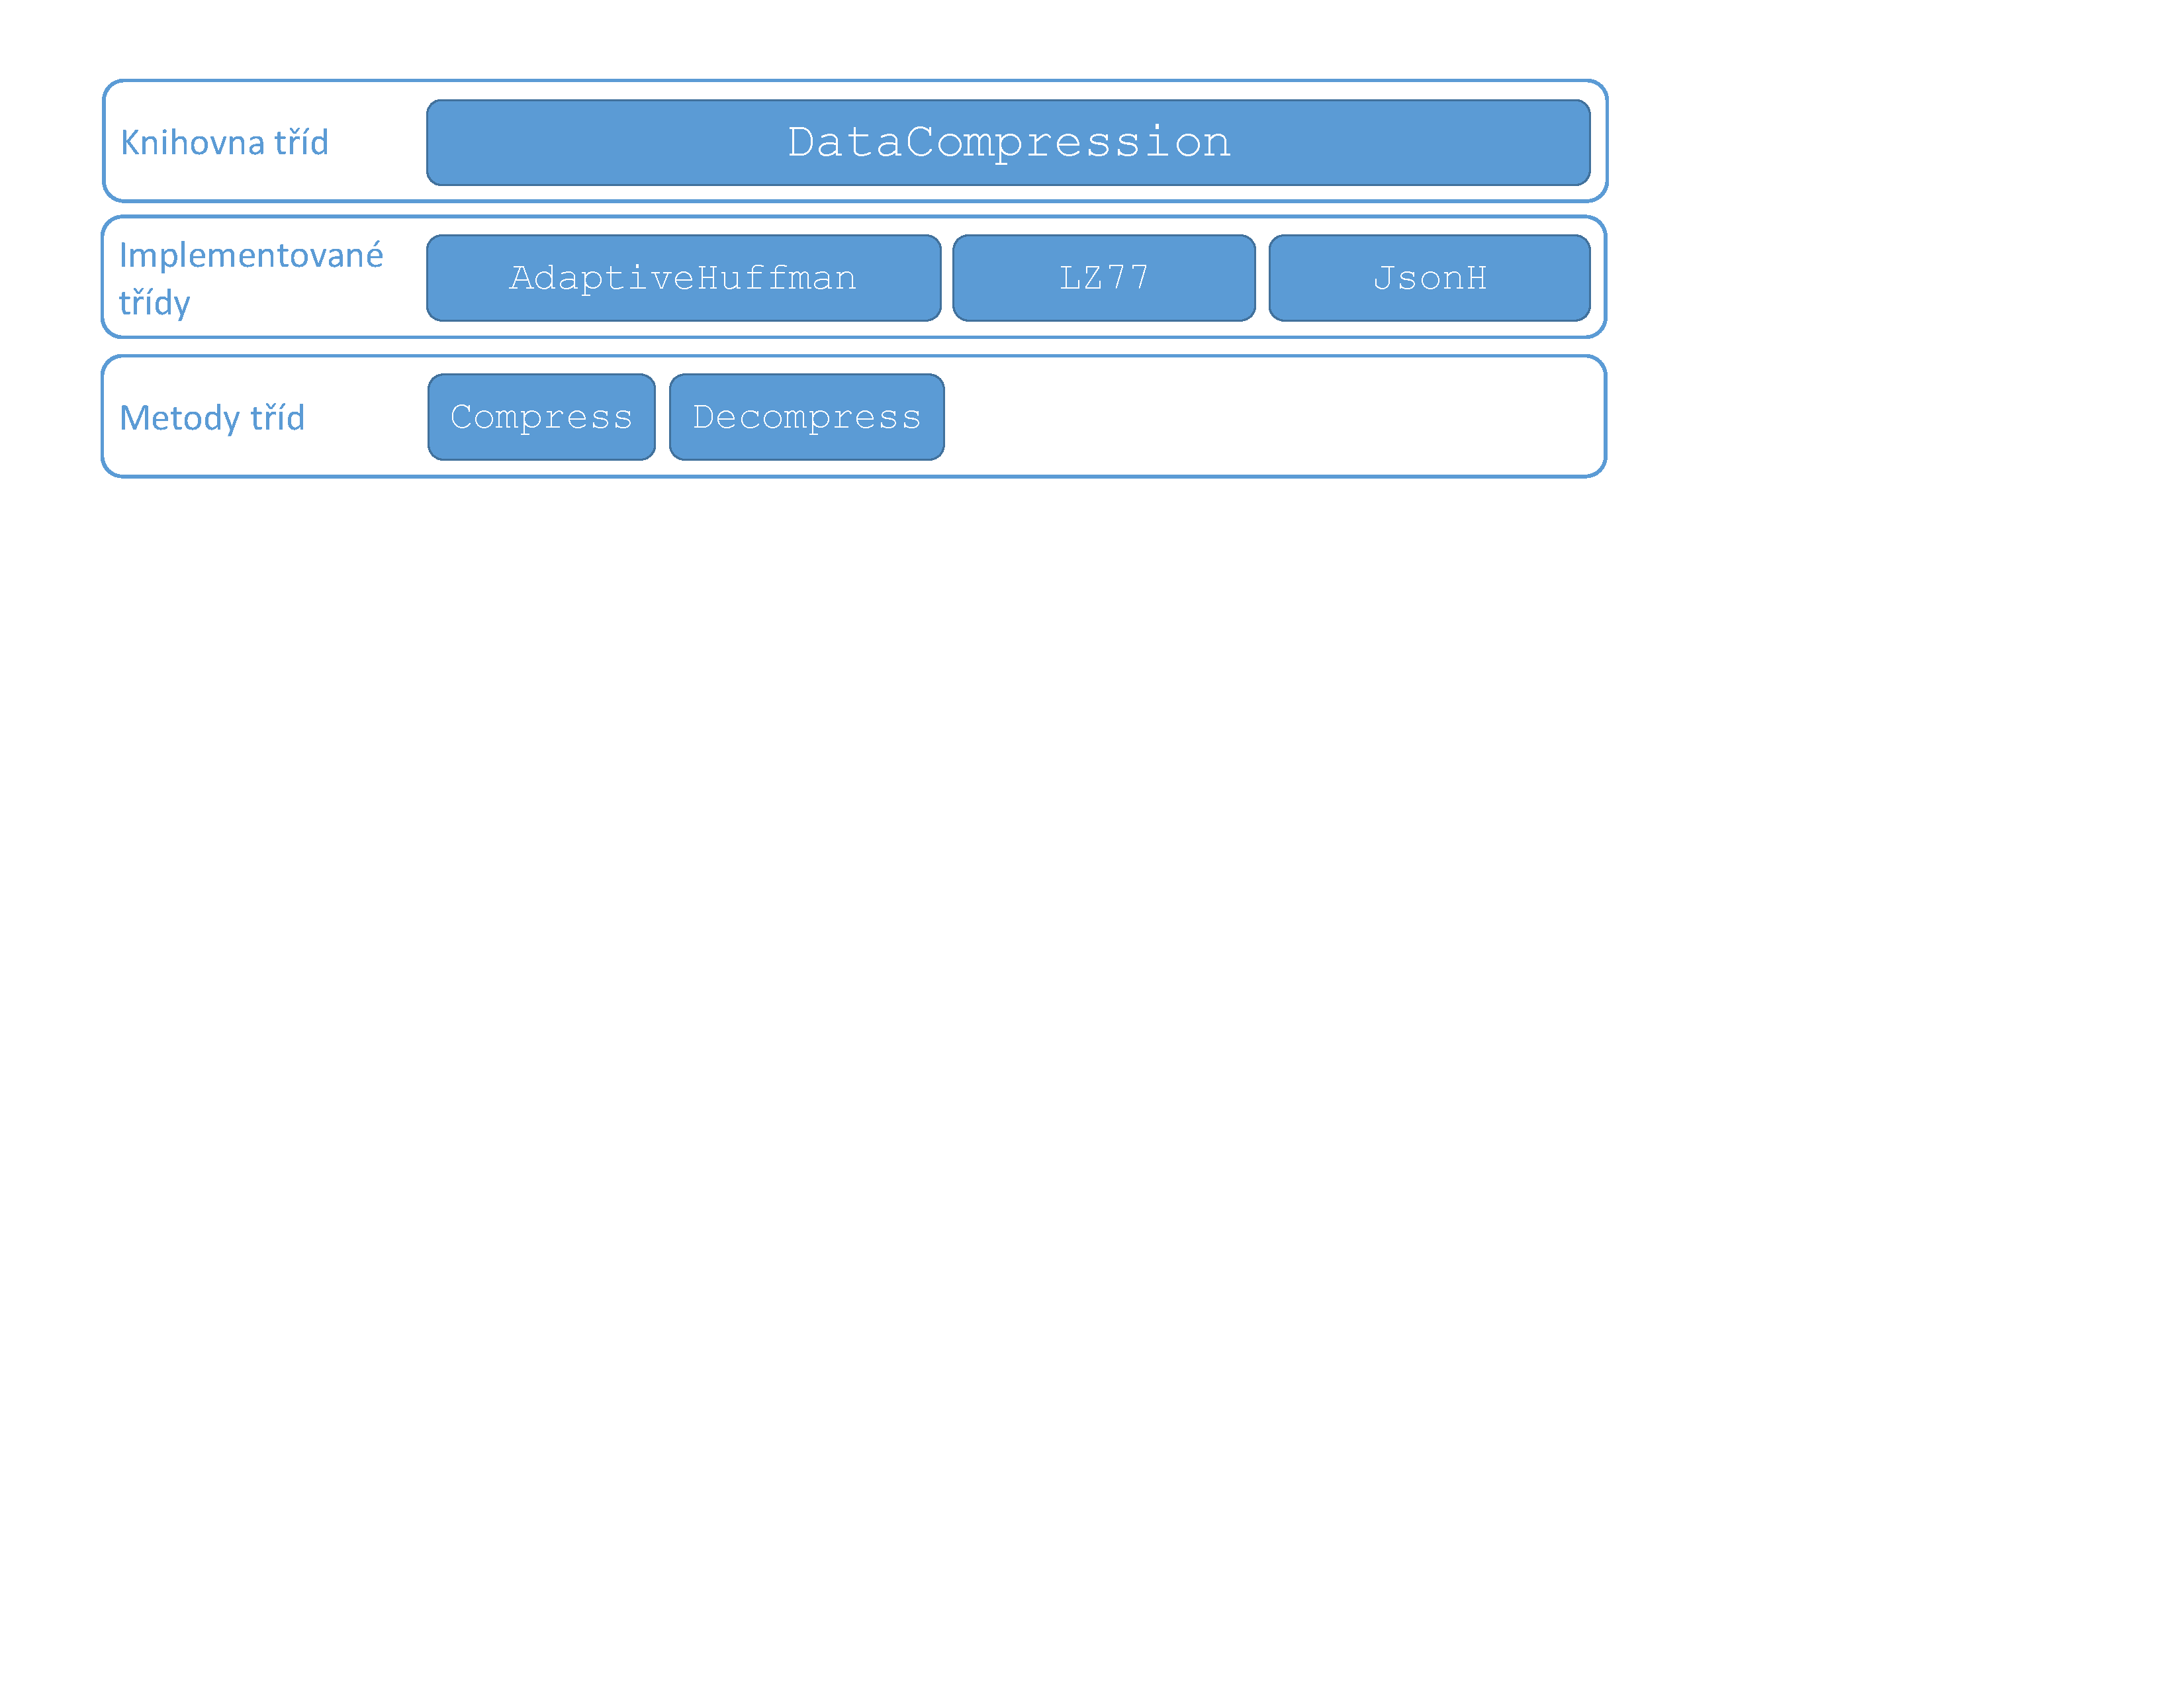
\includegraphics[trim=70 875 415 55, clip, angle=0, width=150mm]{strukturaKnihovny}
\caption{Struktura knihovny kompresních algoritmů}
\label{strukturaKnihovny}
\end{figure}


\section{Vybrané algoritmy}
\subsection{Adaptivní Huffmanovo kódování}
Ze statistických kompresních metod jsem zvolil Jeffreyho S. Vitterovu verzi adaptivního Huffmanova kódování, která je považována za složitější na implementaci, ale proti jiným verzím staví vyváženější stromy a tedy generuje kratší kódová slova. Uživatel má k dispozici třídu \texttt{AdaptiveHuffmanCompressor} s veřejnými metodami \texttt{Compress} a \texttt{Decompress}. 

Jádrem algoritmu je ale třída \texttt{VitterTree}, která implementuje logiku chování stromu. Pro každý přečtený znak je při kompresi zavolána jeho metoda \texttt{AddChar} (viz algoritmus 1), která provede aktualizaci stromu dle algoritmu 2 a vrátí binární kód znaku ve stromu.

\begin{table}[!h]
\centering
\begin{tabular}{l}
\hline
\textbf{Algoritmus 1:} \texttt{AddChar}\\
\hline
\textbf{Vstupní parametry:} ASCII kód znaku \texttt{Z}\\
\textbf{Výstupní parametry:} binární kód vloženého znaku\\
\hline
\texttt{if} strom obsahuje uzel se znakem \texttt{Z}\\
\texttt{begin}\\
\hspace*{5mm}vrať kód uzlu se znakem \texttt{Z}\\
\hspace*{5mm}\texttt{UpdateTree(\texttt{Z})}\\
\texttt{end}\\
\texttt{else}\\
\texttt{begin}\\
\hspace*{5mm}vrať kód uzlu NYT\\
\hspace*{5mm}vrať sedmibitový ASCII kód znaku \texttt{Z}\\
\hspace*{5mm}\texttt{UpdateTree(\texttt{Z})}\\
\texttt{end}\\
\hline
\end{tabular}
\end{table}

\begin{table}[!h]
\centering
\begin{tabular}{l}
\hline
\textbf{Algoritmus 2:} \texttt{UpdateTree}\\
\hline
\textbf{Vstupní parametry:} znak \texttt{Z}\\
\textbf{Výstupní parametry:} nemá\\
\hline
uzel \texttt{U :=} uzel se znakem \texttt{Z}\\
\texttt{while} uzel \texttt{U} není kořen\\
\texttt{begin}\\
\hspace*{5mm}\texttt{if} v bloku existuje uzel s vyšším indexem než má uzel \texttt{U}\\
\hspace*{5mm}\texttt{begin}\\
\hspace*{10mm}prohoď uzel \texttt{U} s uzlem s nejvyšším indexem v bloku\\
\hspace*{5mm}\texttt{end}\\
\hspace*{5mm}inkrementuj počet výskytů v uzlu \texttt{U}\\
\hspace*{5mm}\texttt{U :=} předek uzlu \texttt{U}\\
\texttt{end}\\
\hline
\end{tabular}
\end{table}

Pro účely dekomprese je strom implementován jako deterministický konečný automat. Obsahuje \texttt{ukazatel}, který obsahuje referenci na jeden z uzlů (stav automatu). Na počátku ukazuje \texttt{ukazatel} na kořen a s každým přečteným bitem komprimované zprávy se přesune do následujícího uzlu dle přechodové funkce. Je-li přečten kód uzlu obsahujícího znak, je tento znak vrácen a strom aktualizován. Je-li přečten kód uzlu NYT, načte algoritmus dalších 7 bitů, které reprezentují ASCII kód nového znaku, ten je vložen do stromu a vrácen. Zpracování jednoho bitu kódu provádí metoda \texttt{PushBit} (viz algoritmus 3).

\begin{table}[!h]
\centering
\begin{tabular}{l}
\hline
\textbf{Algoritmus 3:} \texttt{PushBit}\\
\hline
\textbf{Vstupní parametry:} jeden bit kódu \texttt{B}\\
\textbf{Výstupní parametry:} přečtený znak, byl-li v tomto kroku přečten\\
\hline
\texttt{if} čten znak nevyskytující se ve stromě\\
\texttt{begin}\\
\hspace*{5mm}kumuluj 7 bitů\\
\hspace*{5mm}\texttt{if} nakumulováno 7 bitů\\
\hspace*{5mm}\texttt{begin}\\
\hspace*{10mm}vrať přečtený znak \texttt{Z}\\
\hspace*{10mm}\texttt{AddChar(Z)}\\
\hspace*{10mm}přesměruj \texttt{ukazatel} na kořen\\
\hspace*{5mm}\texttt{end}\\
\texttt{end}\\
\texttt{else}\\
\texttt{begin}\\
\hspace*{5mm}dle \texttt{B} přesměruj \texttt{ukazatel} na jeho potomka\\
\hspace*{5mm}\texttt{if} ukazatel je uzel obsahující znak\\
\hspace*{5mm}\texttt{begin}\\
\hspace*{10mm}vrať znak \texttt{Z} v uzlu\\
\hspace*{10mm}\texttt{AddChar(Z)}\\
\hspace*{10mm}přesměruj \texttt{ukazatel} na kořen\\
\hspace*{5mm}\texttt{begin}\\
\hspace*{5mm}\texttt{if} ukazatel je uzel NYT\\
\hspace*{5mm}\texttt{begin}\\
\hspace*{10mm}přesměruj \texttt{ukazatel} na kořen\\
\hspace*{10mm}nastav stav stromu na čtení nového znaku\\
\hspace*{5mm}\texttt{begin}\\
\texttt{end}\\
\hline
\end{tabular}
\end{table}

\subsection{JSONH}
